  \documentclass{beamer}
  \usepackage[utf8]{inputenc}
  \usetheme{Pittsburgh}
 
  \usepackage{algorithm}
  \usepackage{algorithmic}
  \usepackage{bm}
  

  \title{Riemann manifold Hamiltonian Monte Carlo methods}
  \author{Pierre Boyeau \and Baptiste Kerl\'eguer\\}\institute{École Normale Supérieure Paris-Saclay}
  \date{10 janvier 2018}

  \begin{document}

  \begin{frame}
  \titlepage
  \end{frame}
  
  \begin{frame}{Plan}
\tableofcontents
 \end{frame}
  
\AtBeginSection[]
{
\begin{frame}{Plan}
\tableofcontents[currentsection]
 \end{frame}
}
  \section{Context}
  
  \subsection{Hamiltonian Monte Carlo}  
  \begin{frame}{Hamiltonian Monte Carlo Classique}
  \underline{Idée}: Introduction d'une variable auxiliaire $\bm{p}$: 
  
  
  Log-proba négative cible: Hamiltonien: $$ H(\bm{\theta},\bm{p}) = -\mathcal{L}(\bm{\theta}) + \frac{1}{2} \log{(2\pi)^2|\bm{M}|} +\frac{1}{2} \bm{p}^T\bm{M}^{-1}\bm{p} \label{Hamiltonian}$$
  $$ \text{avec } M \text{ une matrice de masse}$$
  \'Equation d'\'evolution : 
  \begin{eqnarray}
  \frac{d\bm{\theta}}{d\tau} = \frac{\partial H}{\partial \bm{p}} \\
  \frac{d\bm{p}}{d\tau} = -\frac{\partial H}{\partial \bm{\theta}}
  \label{evolution}
  \end{eqnarray}  
  
  \end{frame}
  
  \subsection{Variété Riemannienne}
  \begin{frame}{Variété Riemannienne}
  \underline{Idée}: Prendre en compte des arguments de géométrie Riemannienne pour \textit{sampler} $p$:
  $M \rightarrow \bm{\theta}$ $G(\bm{\theta})$.\\
  Nouvelle équation d'évolution:
  \begin{eqnarray}
  \frac{d\bm{\theta}}{d\tau} = G(\bm{\theta})^{-1}\bm{p} \\
  \frac{d\bm{p}}{d\tau} = \nabla_\theta\mathcal{L}(\bm{\theta})-\frac{1}{2}\text{tr}\left(G(\bm{\theta})^{-1}\frac{\partial G(\bm{\theta})}{\partial \bm{\theta}} \right)+\frac{1}{2}\bm{p}^T(\bm{\theta})^{-1}\frac{\partial G(\bm{\theta})}{\partial \bm{\theta}}(\bm{\theta})^{-1}\bm{p}
  \label{evolution}
  \end{eqnarray}
  $\Rightarrow$ Calcul de $G(\bm{\theta})^{-1}$ nécessaire.
  \end{frame}
  
  \begin{frame}{Choix de $G(\bm{\theta})$}
	Prise en compte de la réalité géométrique locale
	
	\begin{itemize}
	\item Espérance de l'information de Fisher
	\item Observation de l'information de Fisher observée
	\item Information de Fisher empirique
	\item Autres tenseurs
	\end{itemize}
		
	  
%  Notre choix de $G(\theta)$ en consid\'erant le problème actuel 
%  $$ G(\beta) = \bm{X}^T\bm{\Lambda X} +\alpha^{-1}\bm{I} $$
  
%  Pour obtenir une variété de courbure constante:
%  $$ G=\bm{X}^T\bm{X}+\alpha^{-1}\bm{I} $$
  
  \end{frame}

  
  
  \subsection{Riemann Manifold Hamiltonian Monte Carlo}
  
  \begin{frame}{RMHMC}
  On suppose qu'on a $\bm{\theta}_n$. Gibbs sampling:
  \begin{enumerate}
    \item Sampler $\bm{p}_{n+1}|\bm{\theta_n} \sim \mathcal{N}(0, G(\bm{\theta}_n))$
    \item Le \textit{proposal} $(\bm{\theta}_{*}, \bm{p}_*)$ est obtenu à l'aide de l'intégrateur de Verlet.
    
    $\bm{\theta}_{*}$ accepté avec probabilité: 
    \begin{align*}
    min(1, \exp[H(\bm{\theta}_n, \bm{p}_{n+1}) 
    - H(\bm{\theta}_*, \bm{p}_*)])
    \end{align*}
    \underline{Interprétation et remarques}
  \end{enumerate}
  \end{frame}  
  
  \begin{frame}{Intégrateur de Verlet}
	Pour assurer un MCMC correct, l'intégration des équations de trajectoire doit être	
	\begin{itemize}
	\item Réversible
	\item Préservation du volume
	\end{itemize}
	
	\begin{align*}
p\left(\tau +\frac{\epsilon}{2}\right)=p\left(\tau\right)-\frac{\epsilon}{2}\nabla_\theta H\left(\theta(\tau\right),p\left(\tau +\frac{\epsilon}{2}\right) \\
\theta(\tau +\epsilon)=\theta(\tau)\\
+\frac{\epsilon}{2}\left[	\nabla_p H\left(\theta\left(\tau\right),p\left(\tau+\frac{\epsilon}{2}\right)\right)+ \nabla_p H\left(\theta\left(\tau+\epsilon\right), p\left(\tau+\frac{\epsilon}{2}\right)\right)\right]\\
p(\tau+\epsilon)=p\left(\tau+\frac{\epsilon}{2}\right)-\frac{\epsilon}{2}\nabla_\theta H\left(\theta\left(\tau+\frac{\epsilon}{2}\right),p\left(\tau+\frac{\epsilon}{2}\right)\right)
	\end{align*}
	
	\begin{align*}
	\end{align*}
	
	\underline{Difficultés soulevées}
  \end{frame}	  
      
  
  \begin{frame}{Algorithme}
  

\begin{algorithmic}
\REQUIRE $G(0)$ $-\mathcal{L}(\theta)$ $p^0$ $\theta^0$
%\ENSURE 
\FOR{$i = 0:N-1$}
\STATE sample $p^{i+1}$ selon $\mathcal{N}(O,G^i)$
\FOR{$j = 1 : Nb_{leapfrogs}$}
\STATE $p_{tempo}=p_\tau$
\FOR{$k = 1 : N_{pointfixe}$}
\STATE $p\left(\tau +\frac{\epsilon}{2}\right)=p\left(\tau\right)-\frac{\epsilon}{2}\nabla_\theta H\left(\theta(\tau),p_{tempo}\right)$
\ENDFOR
\STATE $p\left(\tau +\frac{\epsilon}{2}\right) =p_{tempo}$
\STATE $\theta_{tempo}=\theta(\tau)$
\FOR{$k = 1 : N_{pointfixe}$}
\STATE $\theta(\tau +\epsilon)=\theta(\tau)+\frac{\epsilon}{2}\left[G^{-1}\left(\theta(\tau)\right)+G^{-1}\left(\theta_{tempo}\right)\right]p\left(\tau+\frac{\epsilon}{2}\right)$
\ENDFOR
\STATE $\theta(\tau+\epsilon)=\theta_{tempo}$
\STATE $p(\tau+\epsilon)=p\left(\tau+\frac{\epsilon}{2}\right)-\frac{\epsilon}{2}\nabla_\theta H\left(\theta\left(\tau+\frac{\epsilon}{2}\right),p\left(\tau+\frac{\epsilon}{2}\right)\right)$
\ENDFOR
\ENDFOR
\end{algorithmic}

  \end{frame}
  
  \section{Application: Régression Logistique Bayésienne}
  \begin{frame}{Régression Logistique Bayésienne}
	\underline{Modèle}: 
	\begin{enumerate}
	\item Prior gaussien: $ \beta \sim \mathcal{N}(0,\alpha I) $
	\item Loi $Y|\beta$: modèle de régression logistique classique
\end{enumerate}	  
  
  	Tenseur métrique choisi: information de Fisher $G(\beta)=\bm{X}^T\bm{\Lambda}\bm{X}+\alpha^{-1}I$
  	
  	\underline{Travail réalisé}: Etude comparée de RMHMC et de HMC sur cette tâche et sur données simulées.
  \end{frame}

\subsection{Validation de l'algorithme}
\begin{frame}{Validation de l'algorithme}
   \begin{figure}
   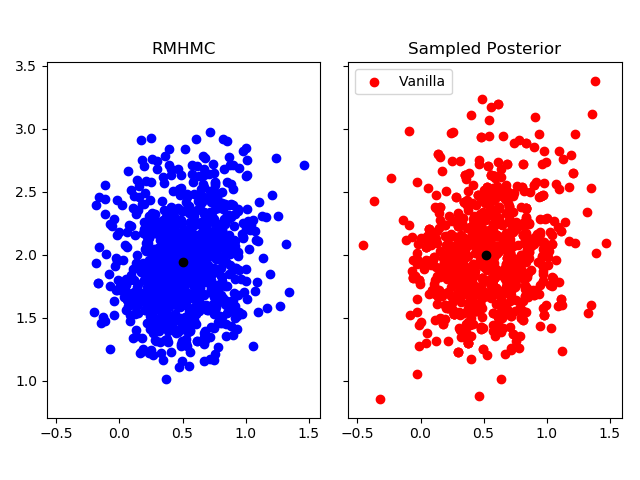
\includegraphics[scale=0.4]{figs/posterior_comparison_100_vs_100.png}
   \end{figure}
\end{frame}

\subsection{Performances sur données simulées}
\begin{frame}{Performances}
	\begin{figure}
	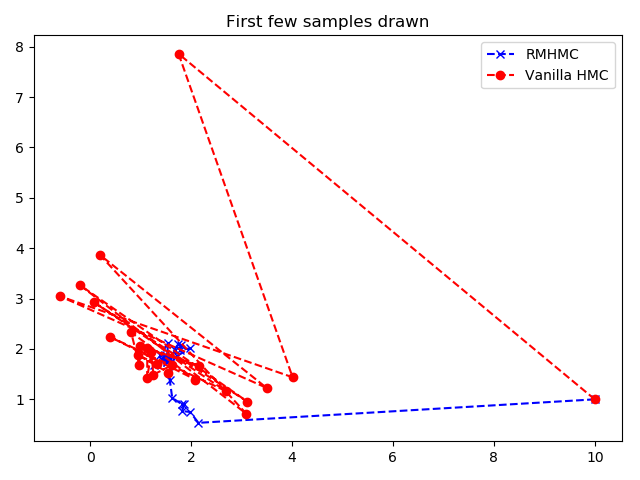
\includegraphics[scale=0.4]{figs/conv_2d_6leaps_vs_100.png}
	\end{figure}
\end{frame}

\begin{frame}{Performances}
	\begin{figure}
	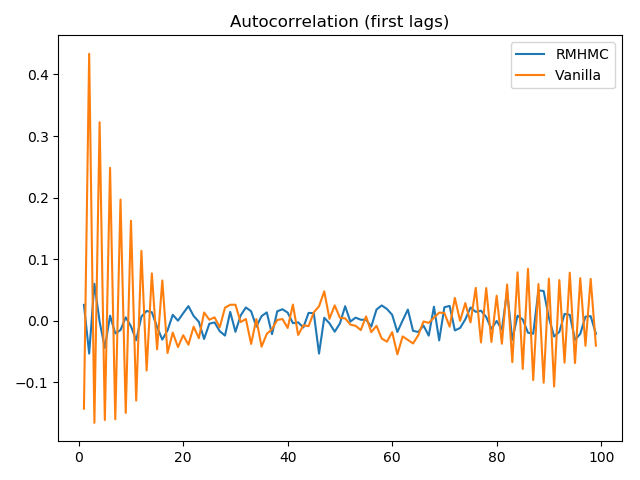
\includegraphics[scale=0.4]{figs/autocorr_mean_100_100.png}
	\end{figure}
\end{frame}

\subsection{Performances sur données réelles}
\begin{frame}{Données réelles}
   \begin{figure}
   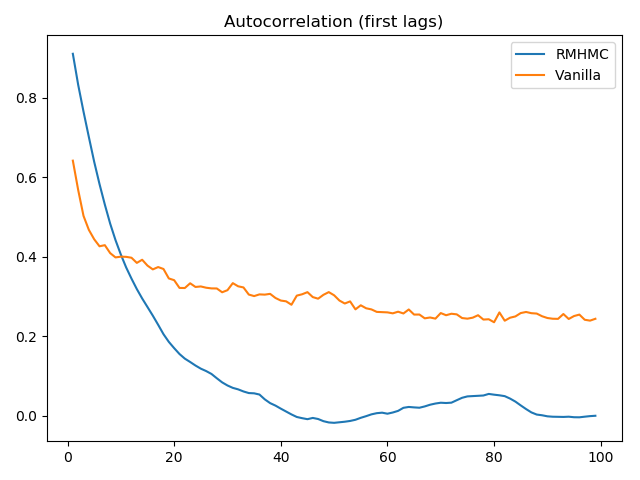
\includegraphics[scale=0.4]{figs/autocorr_real_6_vs_100.png}
   \end{figure}
\end{frame}

\section{Limites et ouvertures}
\begin{frame}{Limites et ouvertures}
\underline{Limites:}
\begin{itemize}
\item Coût computationnel important
\end{itemize}

\underline{Ouverture}
\begin{itemize}
\item Acceptance ratio
\item Choix de $G(\theta)$
\end{itemize}
\end{frame}

  \begin{frame}
  \bibliographystyle{ieee}
  \bibliography{egbib}
  \end{frame}
 

  \end{document}